 Discrete Particle Model simulates particle motion by applying forces and torques which derives from particle-particle interactions and external influences, on the basis of the given contact law. It performs calculations of kinematics that a given particle $i$ exerts on other particle $j$, for each particle in the system, among with the peripheral factors such as gravity and walls. To achieve this results, the particles are assumes to be (1) undeformable - deform therefore implemented as overlap, (2) unbreakable, (3) all internal interactions are due to particle-particle interaction, (4) Each particle pair $i, j$ has only one contact point $c_{ij}$ which the forces and torques act on, and (5) all external forces and torques are either body forces and torques or by interacting with a wall \cite{MercuryDPM}. 

\subsubsection{Contact Laws}
For each particle $i$ on the system, Eq. \ref{eq:force} describes the internal and external forces, and Eq. \ref{eq:torque} describes the torque acting on it \cite{MercuryDPM}:

\begin{equation} \label{eq:force}
    F_i = \sum_{j=1}^{n_p} F_{ij} + \sum_{k=1}^{n_w} F_{ik}^w  + F_i^b
\end{equation}

\begin{equation} \label{eq:torque}
    \tau_i = \sum_{j=1}^{n_p} r_{ij}F_{ij} + \tau_{ij} + \sum_{k=1}^{n_w} r_{ik}F_{ik}^w + \tau_{ik}^w +\tau_{i}^{b} 
\end{equation}

With $F_{ij}$ interparticle forces, $F_{ik}^w$ the interaction force between each wall and the particle, $n_p =$ number of particles, $n_w =$ number of walls, $F_i^b$ body forces i.e., gravity, and $r_{ij}$ as the branch vector, which connects the particle position $r_i$ with the contact point $c_{ij}$ . The same hold for torques equation, with $\tau$ as torque. 

The contact law used in the simulations is the Linear Spring-Dashpot model, which is implemented in MercuryDPM as \texttt{LinearViscoelasticSpecies}. It defines the interaction between two particles $i$ and $j$ as a damped harmonic oscillators \cite{LSD-info}:

\begin{equation}
    F_{ij}^n=\begin{cases}
        k_n \delta_{ij}^n + \gamma_n v_{ij}^n &\text{if } \, \delta_{ij}^n > 0, \\
        0 \quad &\text{else, } \,   \\
   \end{cases}
\end{equation}

In this equation, $k_n > 0$ represents spring stiffness, $\gamma_n \geq 0$ represents the damping coefficient, $v_n$ the normal vector, and $\delta_{ij}^n$ is the overlap between the particles. Two particles interact with each other if and only if they overlap. This contact model is simple, has an analytic solution and less computationally expensive \cite{NAVARRO2013}, while also suitable for large particles \cite{MercuryDPM}. 


\subsubsection{Angle of Repose}
Angle of Repose (AoR) is one of the most important bulk parameters to describe the characteristics of Granular Material. Despite having a generic name, definitions of AoR differs vividly, subject to different applications and behaviors \cite{BEAKAWIALHASHEMI2018397}. In the context of this Assignment, two different AoR will be discussed: Static and Dynamic Angle of Repose. 

\begin{figure}[H]
    \centering
    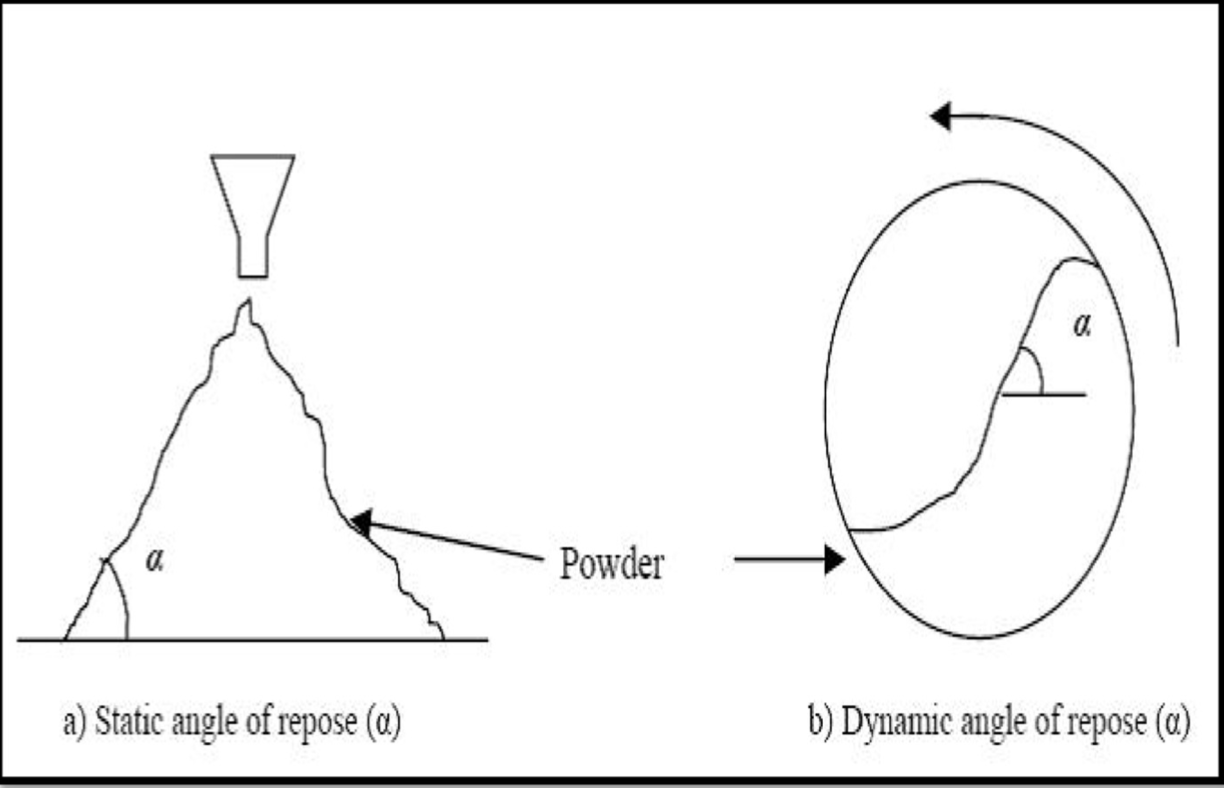
\includegraphics[scale=0.6]{StaticDynamicAoR.png}
    \caption{Static and Dynamic Angle of Repose \cite{PhysRevLett.82.1156}.}
    \label{fig:StaticDynamicAoR}
\end{figure}


\paragraph{Static Angle of Repose and heap shape measurement} \label{section:staticAoR}

Static AoR, as described in Fig. \ref{fig:StaticDynamicAoR}a, is defined as the angle that granular solids forms when it piled with a flat surface, and is essential to characterise the coarseness and smootheness of materials. This in turn can help designing a process involved with the material - lower static AoR implies more flowable and thus easier to transport with less energy \cite{TEFERRA201945}. 

In MercuryDPM, Static AoR is measured by a hollow cylinder simulation. A flat surface is placed at the bottom, and then a cylinder is positioned right on top. After that, the particles are poured into the cylinder, rested, and then the cylinder is removed, which will results in a cone-shaped heap of particles. After the heap is rested, the center of mass of the heap is calculated to determine the height of the cone. The angle results from $\arctan(height/diameter)$ is the static AoR. The key point here is to let the heap of particle comes to a fully rested state, i.e., the kinetic energy is negligible compared to the potential energy. This is proved challenging for simulations with low coefficient of friction - which led to an unstable heap. 

\paragraph{Dynamic Angle of Repose and powder cohesion measurement}


